\chapter{Stand der Technik}

\section{Schachcomputer}
Ein erster Meilenstein wurde hier mit Deep Blue, einem Schachcomputer von IBM geschaffen. Ziel des Team war es, der beste
Schachspieler der Welt zu schlagen. Der erste Versuch scheitetere im Februar 1996 in Philadelphia gegen Garry Kasparov mit 4-2.
Im Mai 1997 kam es zu einem berühmten Rematch, welches im Equitable Center in New York ausgetragen wurde.
Hier schlagte Deep Blue Kasparov 3.5-2.5 (\cite{deepBlueIbm}).

Dies war eine grosse Sensation, denn Garry Kasparov war 1985 bis 2000 Classical World Champion (\cite{worldChessChampion})
und gilt nach \href{chess.com}{chess.com}, wegen seinen Erfolgen als bester Schachspieler aller Zeiten (\cite{bestChessPlayerOfAllTime}).

\subsection{ELO}
Mittlerweile hat sich der Abstand zwischen Mensch und Maschine deutlich erhöht. Dies ist dies beispielsweise anhand des \gls{glos:elo}'s zu sehen.

Die offizielle Weltrangliste für die menschliche Spieler ist die von der \gls{glos:fide}. Ebenfalls wird hier die \gls{glos:elo}
von allen Schachspielern verfolgt. Magnus Carlsen hält im Classical Chess aktuell (Stand März 2026) die höchste \gls{glos:elo} mit 2840.
Ebenfalls ist er die Person mit der jemals höchst gemessenen \gls{glos:elo} im Mai 2014 mit 2882 (\cite{magnusFide}).

Auf der anderer Seite gibt es mehrere Ranglisten für Schachcomputer. Die bekanntensten sind hier \gls{glos:ccrl} sowie \gls{glos:cegt}. \\
Da die \gls



In ihrer Statistik vom 28 Februar 2026, haben Sie die Elo mittels


\subsection{Schachtuniere für Computer}
Die Schachcomputer haben sich seither weiterentwickelt und es hat unterschiedliche Gruppierungen gebildet, die Schachcomputer messen
und gegeneinander antreten lassen. Bekannte Organisationen sind hier \gls{glos:ccrl}, \gls{glos:cegt} sowie \gls{glos:tcec}.

Auffällig ist es, dass \gls{glos:stockfish} Stand März 2026 in vielen unterschiedlichen Formaten und Tunieren
die Nase vorne hat und vielfach die höchste \gls{glos:elo} erreicht hat: \cite{ccrlRating} \cite{cegtRating} .

Wichtig ist jedoch, dass die daraus erstellte \gls{glos:elo} lassen sich nicht untereinander vergleichen lässt. Hier werden
je nach Organisation unterschiedliche Berechnungen verwendet. \\
Ebenfalls lässt sich die \gls{glos:elo} nicht mit einer menschlichen, wie der der offizielle Weltrangliste für die
menschliche Spieler ist die von der \gls{glos:fide} vergleichen. \\
Dist



- Bayesian-Elo
- Ordo v1.0.9 cget


- der beste schach computer, vergleich elo von besten schachspieler


es existieren eigene schachtuniere für computer, sodass sie sich untereinander messen können


\subsection{Stockfish}
stockfish ist opensource einer der bekanntesten


\section{Algorithmen}
\subsection{Minimax}
Der Minimax-Algorithmus wird in der Spieltheorie verwendet, um den optimalen Zug für einen Spieler zu finden, angenommen der Gegner spielt auch optimal.
Dieser Algorithmus wird meist für rundenbasierte Nullsummenspiele mit 2 Spieler verwendet.
Der Algorithmus versucht den maximalen Verlust des Spielers zu minimieren - daher der name Minimax.
Mit dieser Logik soll der beste Zug/Pfad für den Spieler gefunden werden, auch wenn der Gegner optimal spielt.

Der Algorithmus hat in nicht-Nullsummenspielen auch eine alternative Version, Maximin genannt, wobei der minimale Gewinn des Spielers maximiert wird.
In Nullsummenspielen sind diese zwei Logiken gleich, in nicht-Nullsummenspielen jedoch nicht.

Da Schach ein rundenbasiertes Nullsummenspiel mit 2 Spielern ist, eignet sich dieser Algorithmus sehr gut um die besten Züge eines Spielers zu berechnen.

\begin{figure}[H]
    \centering
    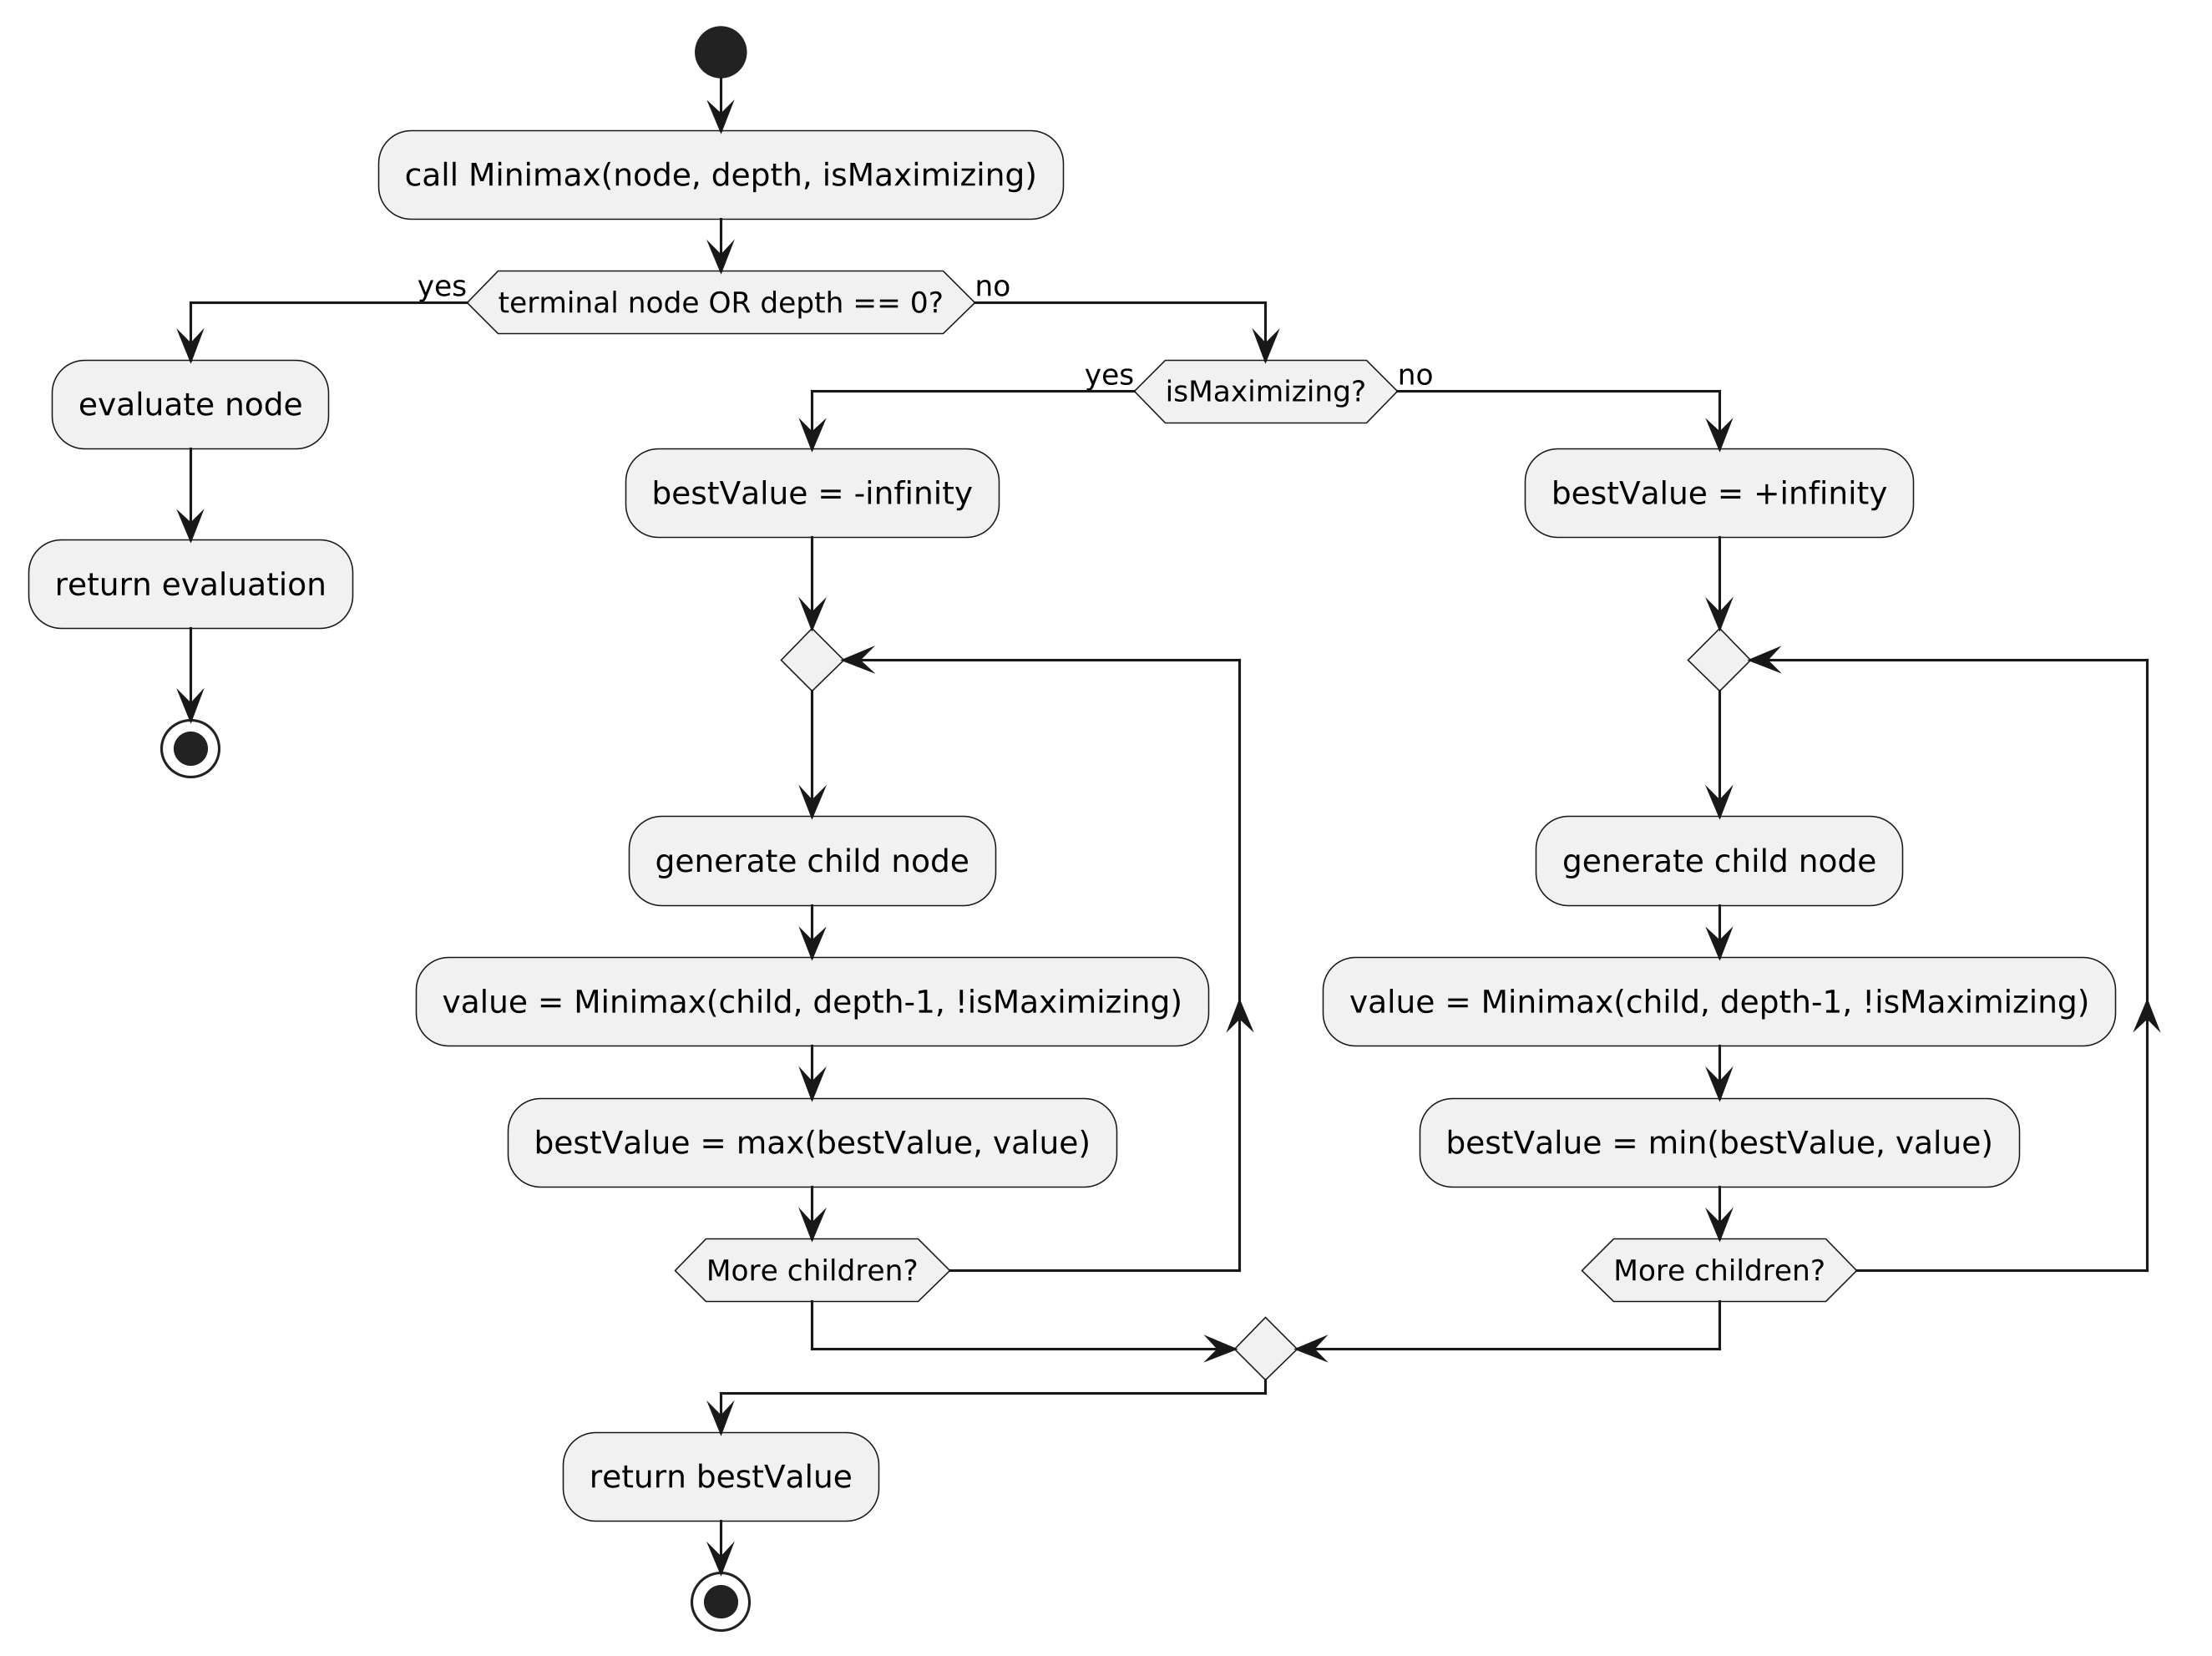
\includegraphics[width=\linewidth]{generated-diagrams/general-minimax}
    \caption{Ablaufdiagramm für Minimax}
    \label{fig:minimax-flowchart}
\end{figure}

Der Algorithmus kann zu Visualisierungszwecken als Baum mit einem Tiefensuchverfahren dargestellt werden.
Ausgenommen der Tiefe 0 (Baumwurzel), stellt jede Tiefe alle Zustände des Spieles dar, welche ein Spieler erzeugen kann.
Somit sind in der Tiefe 1 alle Zustände enthalten, die der Spieler 1 erzeugen kann.
Die Tiefe 2 stellt alle Zustände dar, die Spieler 2 anschliessend erreichen kann.
\begin{figure}[H]
    \centering
    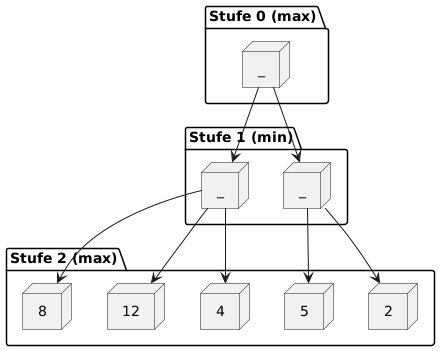
\includegraphics[width=\linewidth]{generated-diagrams/general-minimax-tree-example-0}
    \caption{Minimax Beispielbaum - Ausgangslage}
    \label{fig:minimax-tree-0}
\end{figure}

Dieser Baum enthält 5 Endzustände (unterste Knoten).
Beim Durchlaufen des Baums wird die Vergleichsfunktion immer zwischen min und max umgeschaltet.
Der Baum wird zuerst zu einem Endzustand durchgelaufen, der Zustand wird gemerkt und danach zum übergeordneten Knoten (Entscheidungsknoten) zurückverfolgt.
So werden alle Kinderknoten des vorherigen Entscheidungsknoten traversiert und die Zustände mit der entsprechenden Vergleichsfunktion (hier min) verglichen.

\begin{figure}[H]
    \centering
    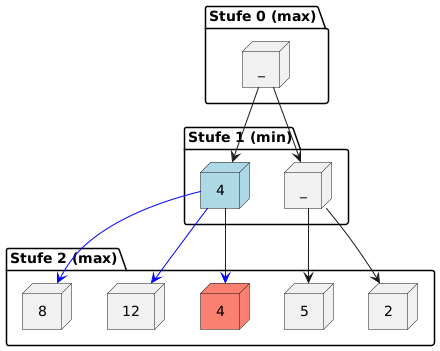
\includegraphics[width=\linewidth]{generated-diagrams/general-minimax-tree-example-1}
    \caption{Minimax Beispielbaum - Schritt 1}
    \label{fig:minimax-tree-1}
\end{figure}

Als nächstes werden alle Entscheidungsknoten der gleichen Ebene auf die gleiche Art berechnet:

\begin{figure}[H]
    \centering
    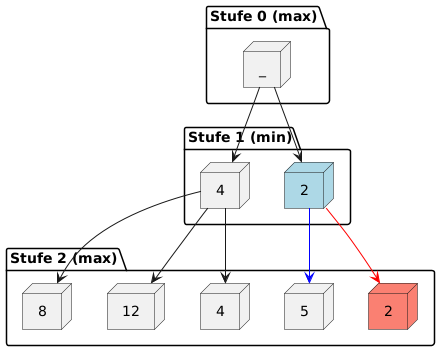
\includegraphics[width=\linewidth]{generated-diagrams/general-minimax-tree-example-2}
    \caption{Minimax Beispielbaum - Schritt 2}
    \label{fig:minimax-tree-2}
\end{figure}

Als letztes wird noch die oberste Ebene auf die gleiche Art berechnet, diesmal wird jedoch der Maximalwert berechnet.

\begin{figure}[H]
    \centering
    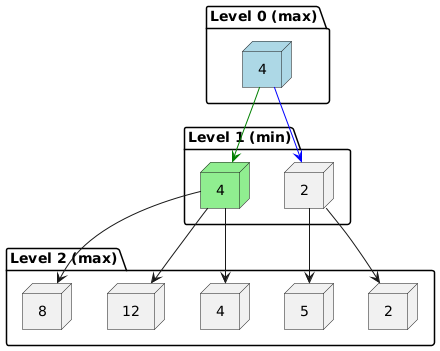
\includegraphics[width=\linewidth]{generated-diagrams/general-minimax-tree-example-3}
    \caption{Minimax Beispielbaum - Schritt 3}
    \label{fig:minimax-tree-3}
\end{figure}

Das Endresultat kann mit der folgenden Abbildung zusammengefasst werden:

\begin{figure}[H]
    \centering
    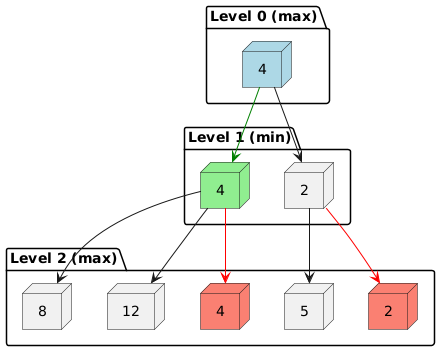
\includegraphics[width=\linewidth]{generated-diagrams/general-minimax-tree-example}
    \caption{Minimax Beispielbaum - Zusammengefasst}
    \label{fig:minimax-tree}
\end{figure}

\subsection{Alpha-Beta-Pruning}
Alpha-Beta-Pruning ist eine Optimierung des Minimax-Algorithmus, wobei Knoten, die das Ergebnis nicht beeinflussen, abgeschnitten werden.

Wir haben zuvor gesehen, dass mit jeder Tiefe des Baums im Minimax-Algorithmus die Anzahl der möglichen Zustände sehr stark ansteigt.
Diese Optimierung versucht die Berechnungszeit der optimalen Züge zu beschleunigen, indem gewisse Pfade komplett übersprungen werden.
Die Entscheidung, ob ein Pfad übersprungen werden kann oder nicht ist sehr von der Reihenfolge der Auswertung abhängig.
Je früher der beste Zustand ausgewertet wird, desto mehr Pfade können übersprungen werden.

In der Abbildung~\ref{fig:minimax-alpha-beta-tree-0} ist die Ausgangslage für das nächste Beispiel zu sehen.
\begin{figure}[H]
    \centering
    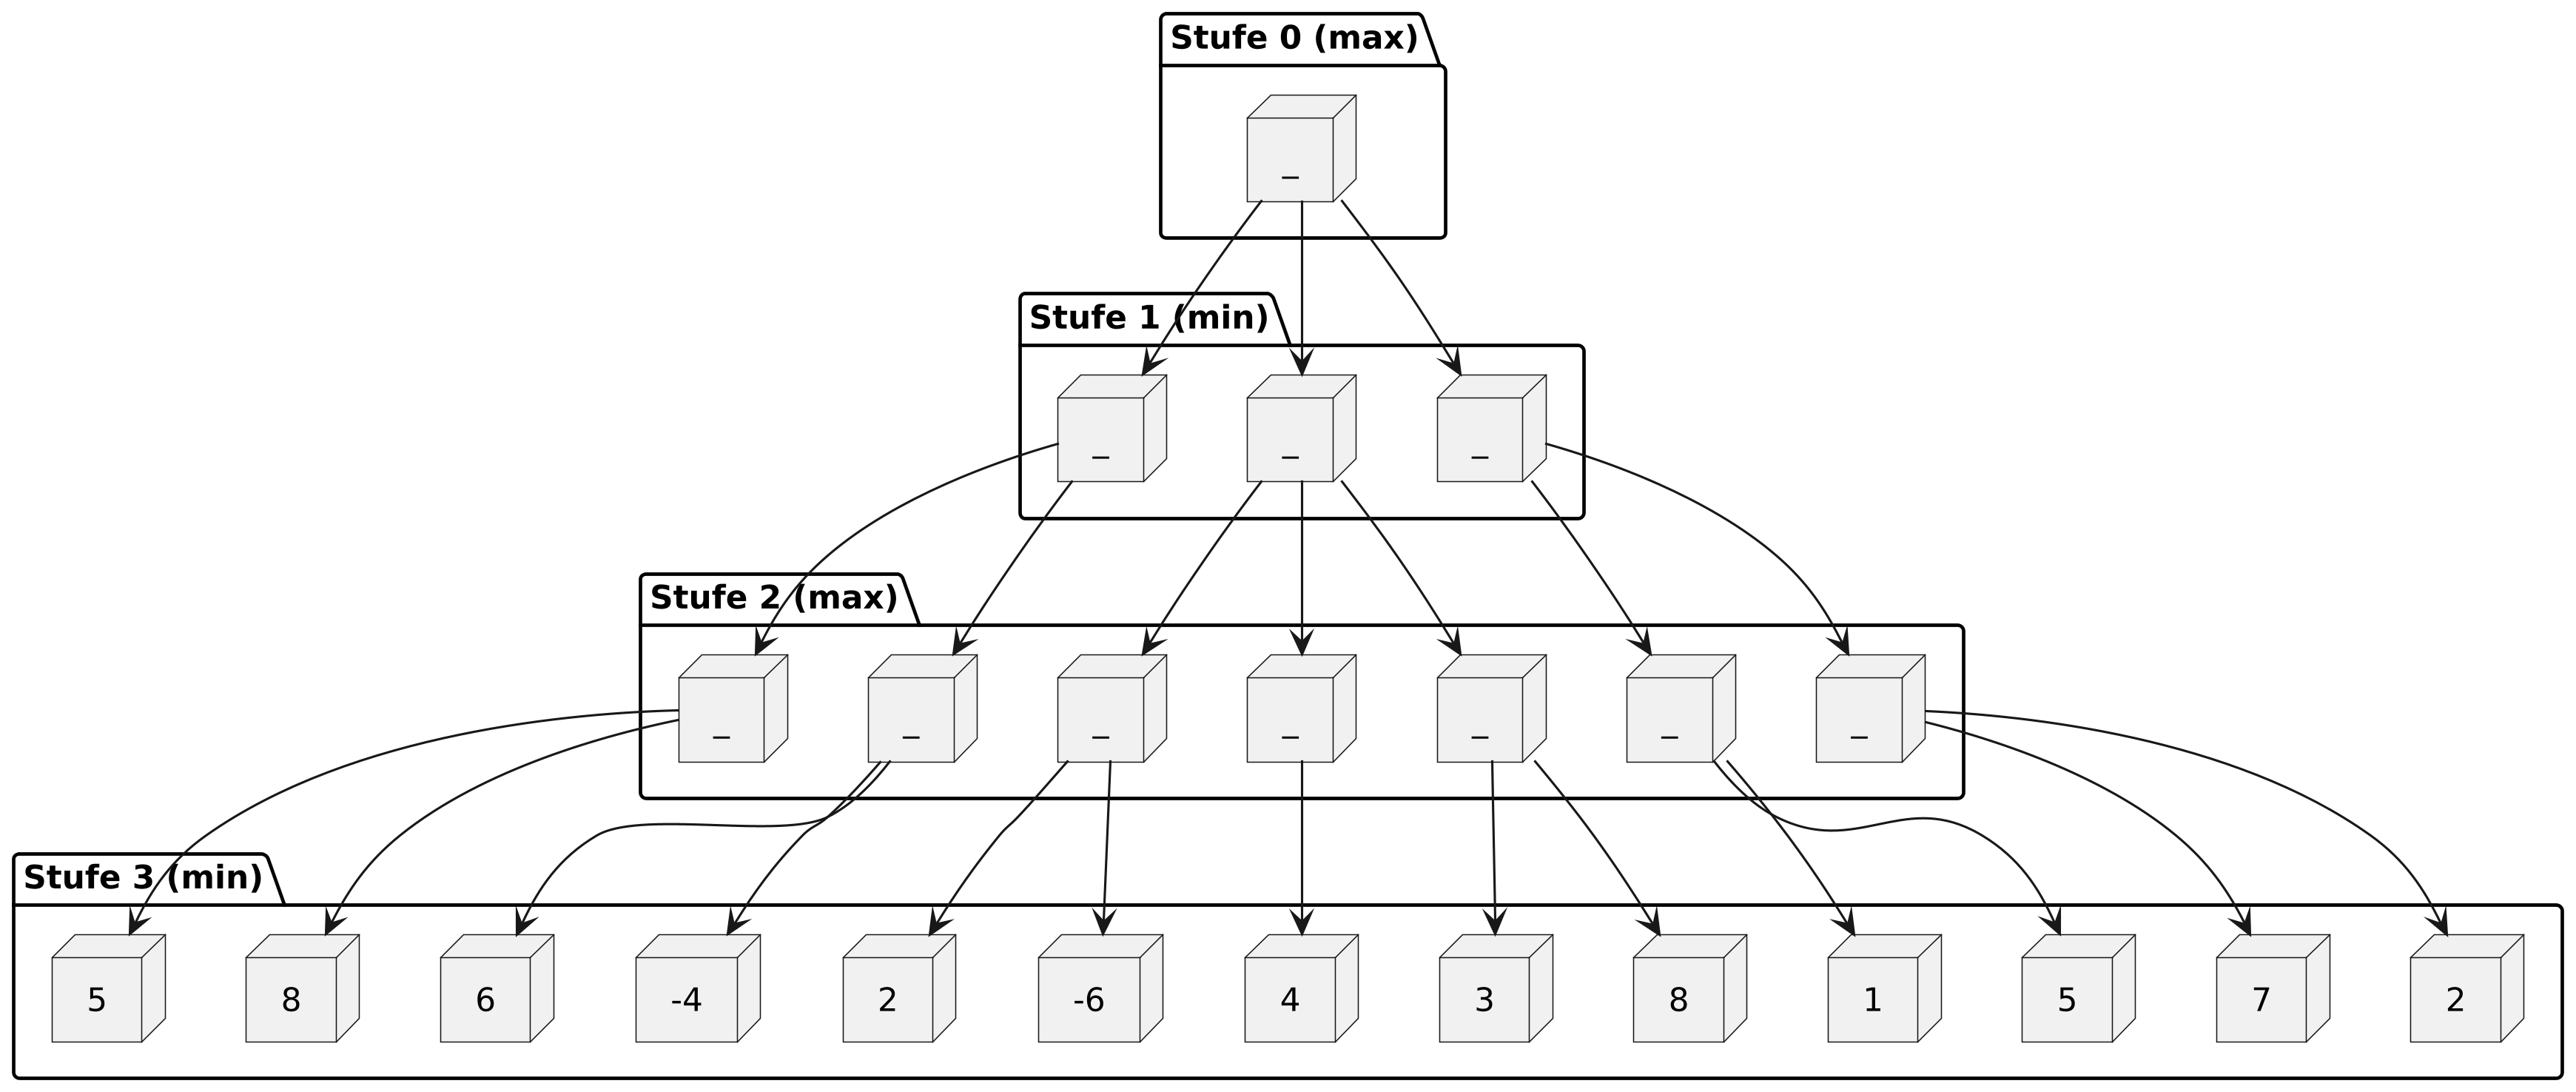
\includegraphics[width=\linewidth]{generated-diagrams/general-alpha-beta-tree-example-0}
    \caption{Minimax Alpha-Beta Beispielbaum - Ausgangslage}
    \label{fig:minimax-alpha-beta-tree-0}
\end{figure}

Hier muss die komplette linke Seite des Baumes durchgelaufen werden, ohne dass eine Alpha-Beta Pruning Optimierung gemacht werden kann.
Im linken Teil des mittleren Teil-Baumes wird Stufe 2 auf die gleiche Art bestimmt.
\begin{figure}[H]
    \centering
    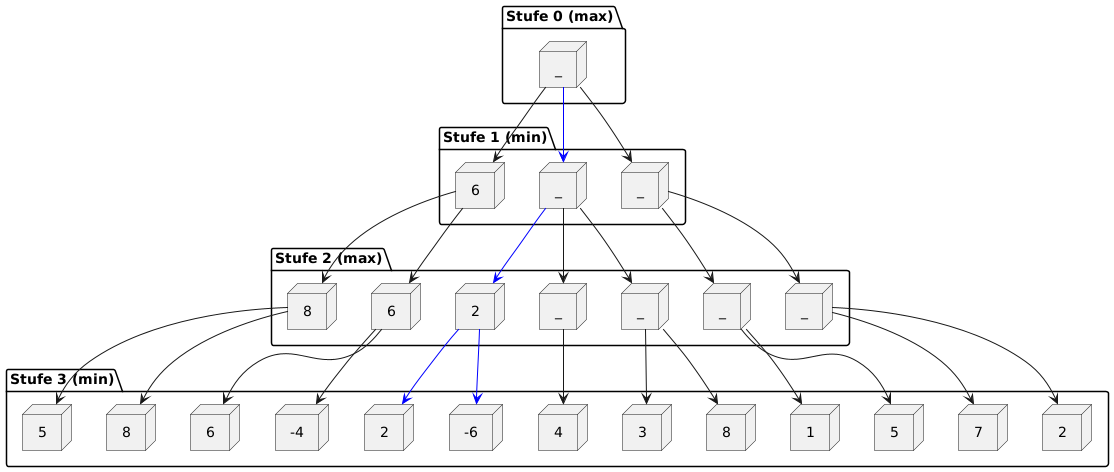
\includegraphics[width=\linewidth]{generated-diagrams/general-alpha-beta-tree-example-1}
    \caption{Minimax Alpha-Beta Beispielbaum - Schritt 1}
    \label{fig:minimax-alpha-beta-tree-1}
\end{figure}

Da Stufe 2 hier den Wert 2 liefert, und die übergeordnete Stufe einen Minimalwert sucht, kann hier provisorisch festgestellt werden, dass die Stufe 1 hier einen Wert liefern wird, der kleiner oder gleich 2 ist.
Die Stufe 0 hingegen sucht einen Maximalwert.
Zwischen 6 und einem Wert der kleiner oder gleich 2 ist, wird der Wert 6 genommen.
Somit kann festgestellt werden, dass es keine Rolle spielt welche Werte in den Stufen 2 und 3 sich im restlichen Teil des mittleren Teil-Baumes befinden, da diese Werte sowieso nicht genommen werden.
\begin{figure}[H]
    \centering
    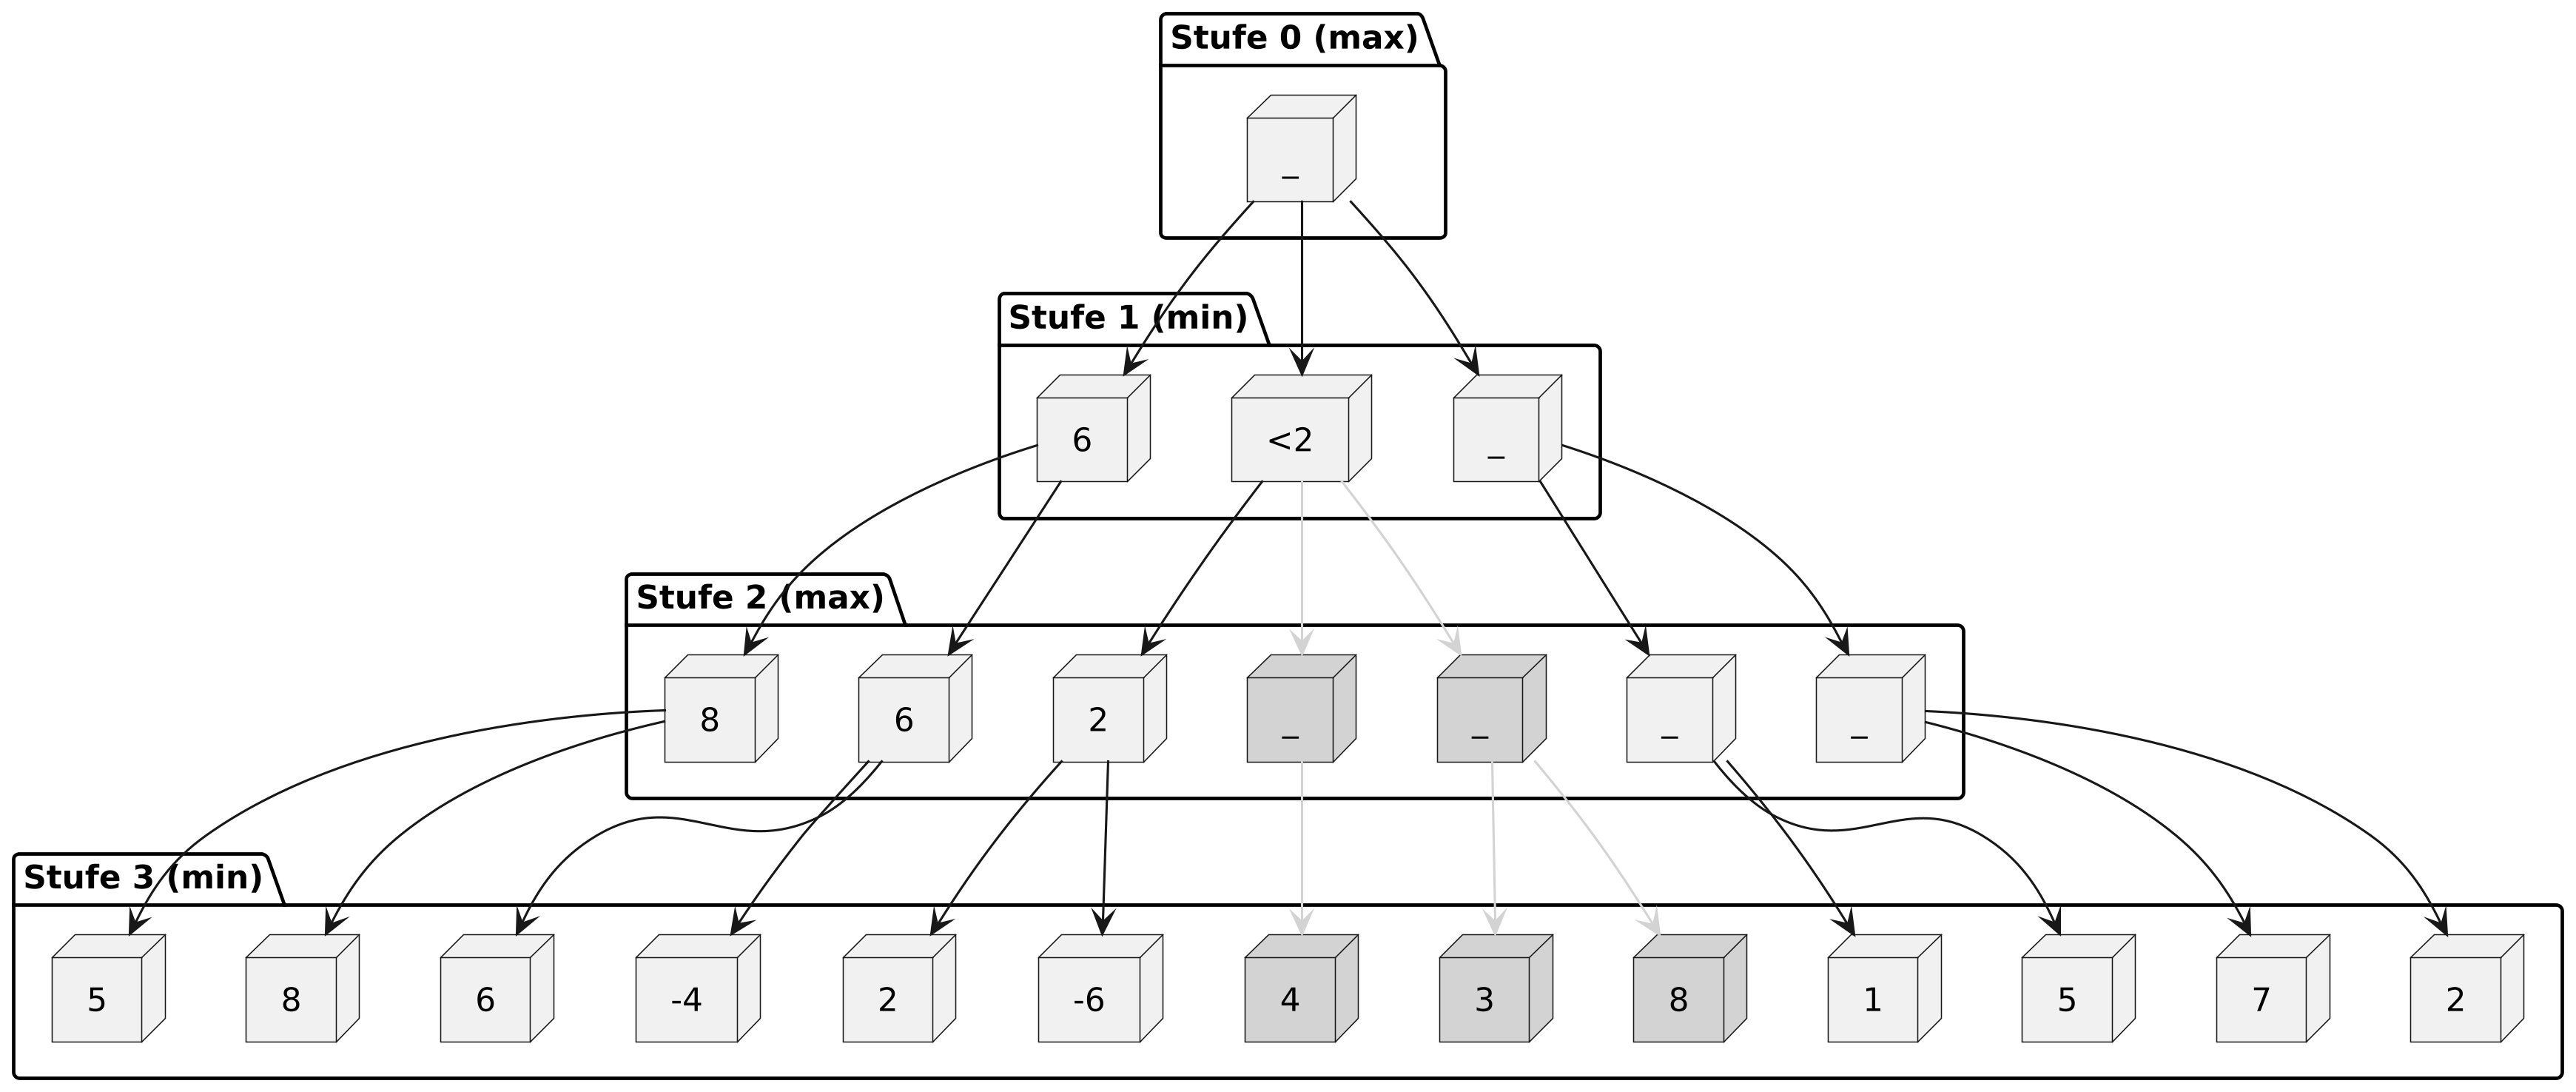
\includegraphics[width=\linewidth]{generated-diagrams/general-alpha-beta-tree-example-2}
    \caption{Minimax Alpha-Beta Beispielbaum - Schritt 2}
    \label{fig:minimax-alpha-beta-tree-2}
\end{figure}

Die gleiche Logik wird auch an die rechte Seite des Baumes angewandt.
\begin{figure}[H]
    \centering
    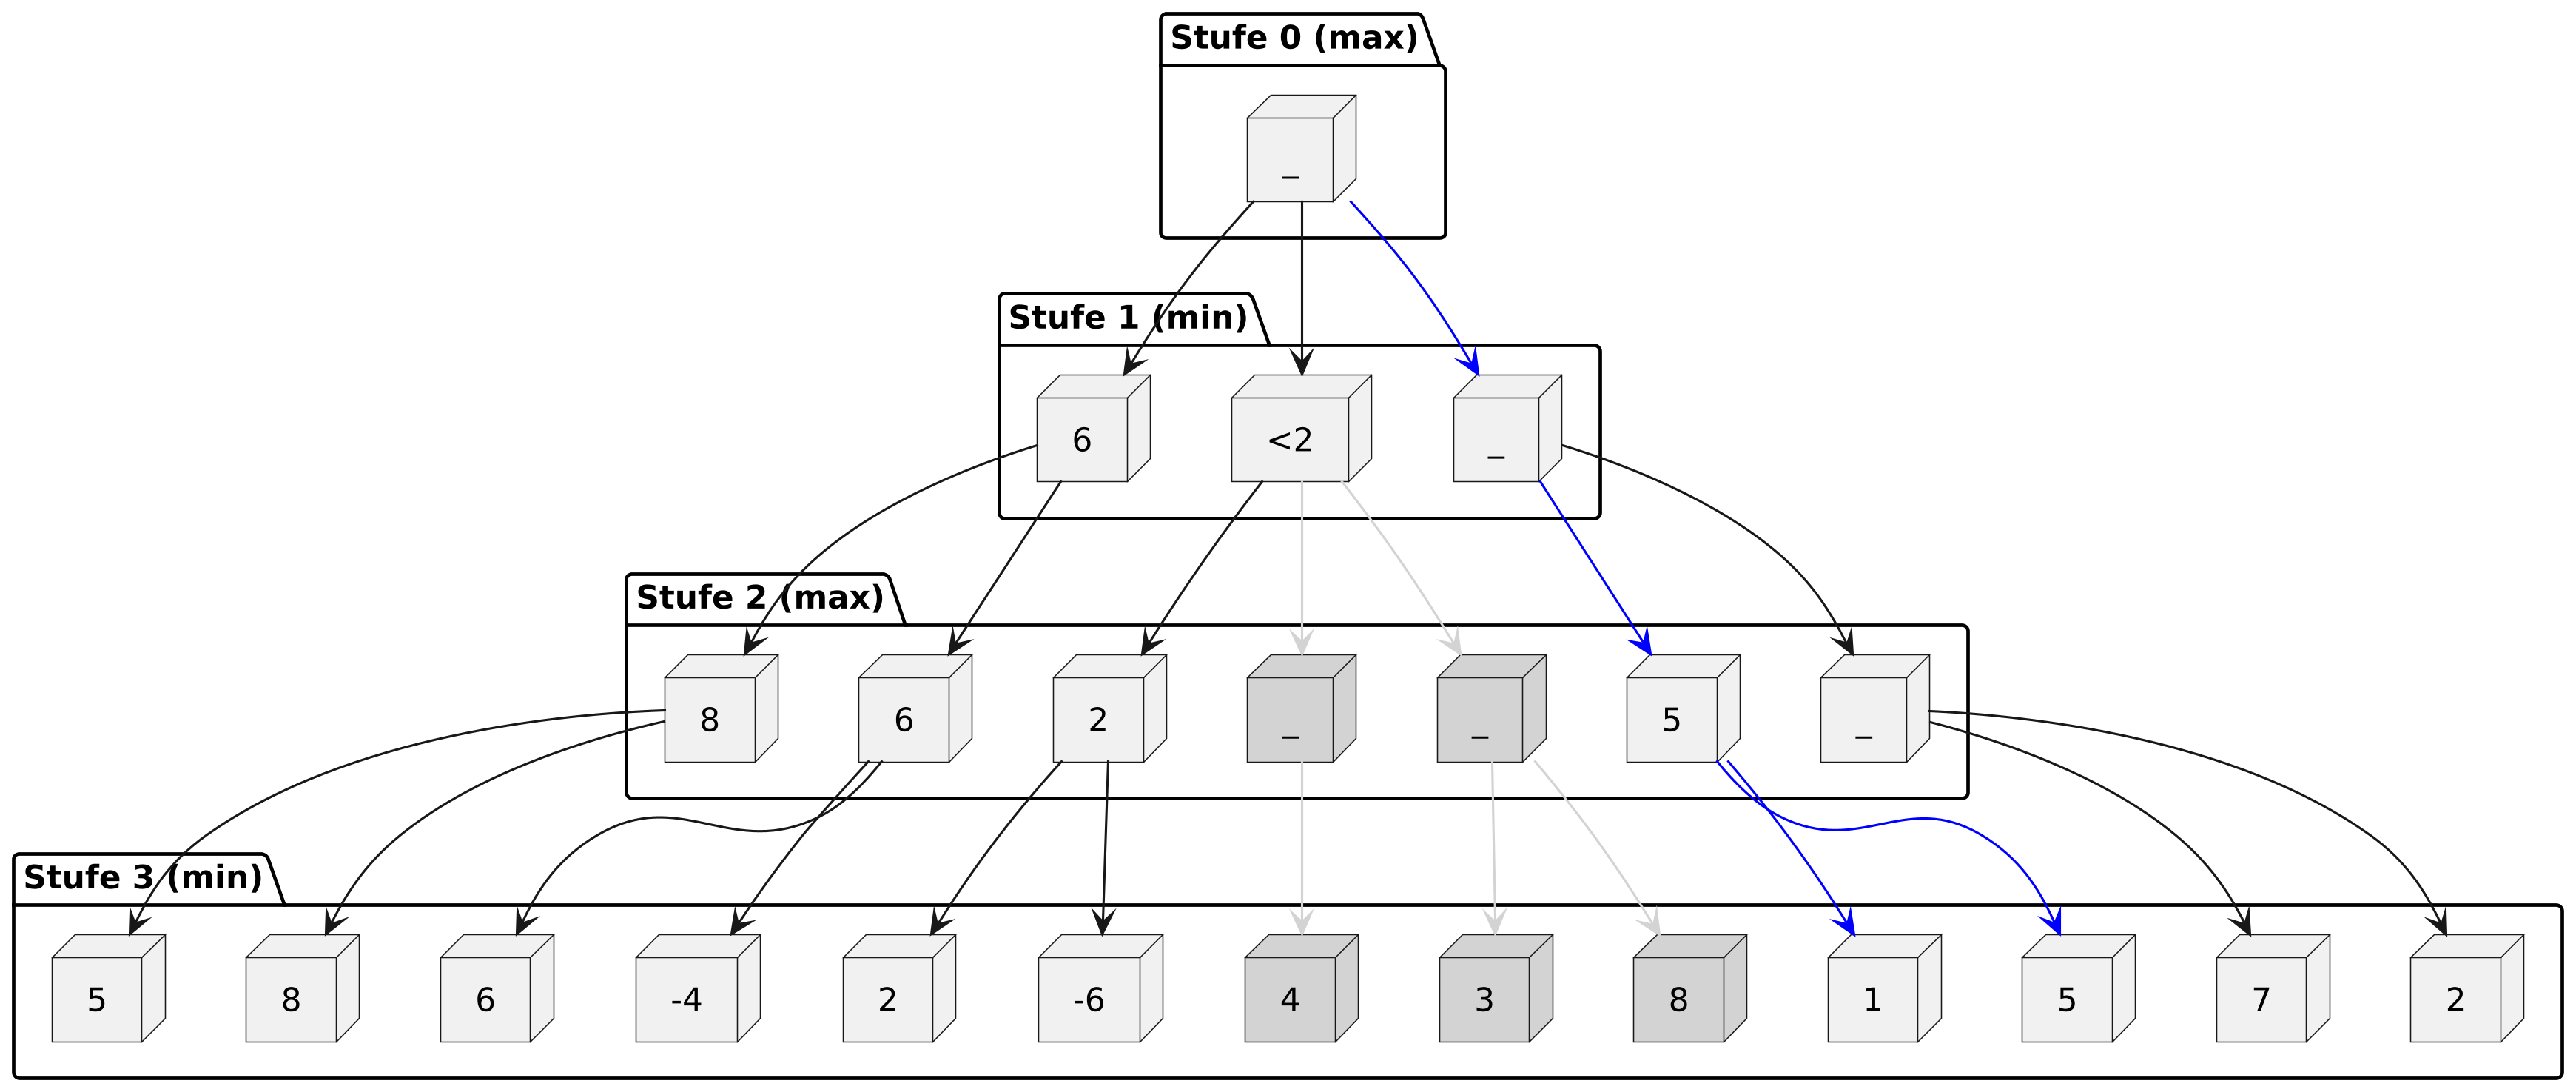
\includegraphics[width=\linewidth]{generated-diagrams/general-alpha-beta-tree-example-3}
    \caption{Minimax Alpha-Beta Beispielbaum - Schritt 3}
    \label{fig:minimax-alpha-beta-tree-3}
\end{figure}

Auf dieser Seite ergibt sich die gleiche Optimierungsmöglichkeit.
\begin{figure}[H]
    \centering
    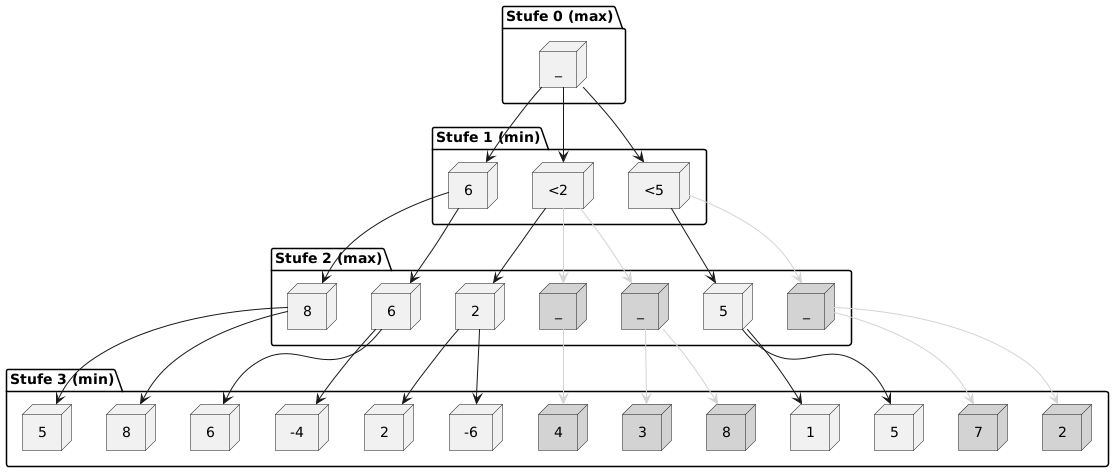
\includegraphics[width=\linewidth]{generated-diagrams/general-alpha-beta-tree-example-4}
    \caption{Minimax Alpha-Beta Beispielbaum - Schritt 4}
    \label{fig:minimax-alpha-beta-tree-4}
\end{figure}

Falls hier die Zustände in einer anderen Reihenfolge wären, z.B., wie in der Abbildung~\ref{fig:minimax-alpha-beta-tree-5}, müsste die ganze Seite traversiert werden und es könnte keine Optimierung stattfinden.
\begin{figure}[H]
    \centering
    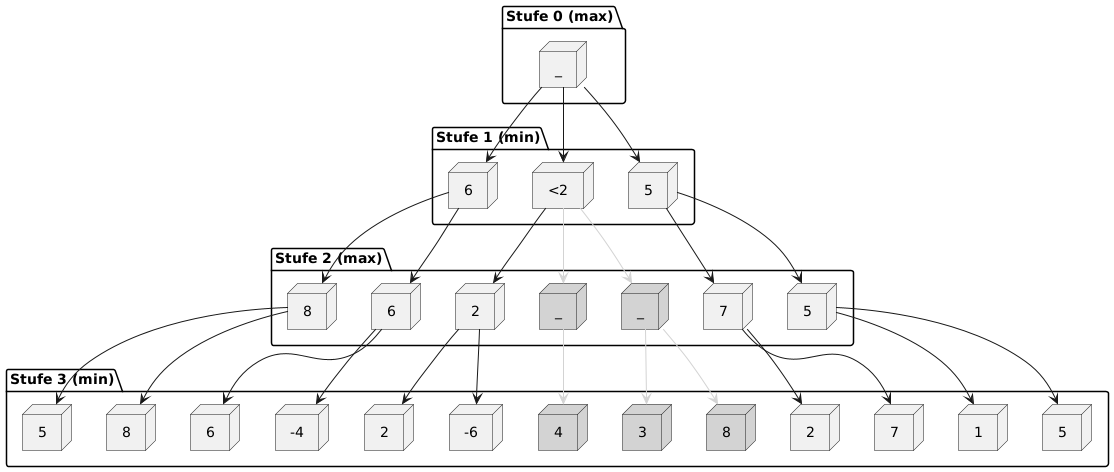
\includegraphics[width=\linewidth]{generated-diagrams/general-alpha-beta-tree-example-5}
    \caption{Minimax Alpha-Beta Beispielbaum - Alternative Reihenfolge}
    \label{fig:minimax-alpha-beta-tree-5}
\end{figure}

Das Ergebnis des Minimax-Algorithmus mit Alpha-Beta-Pruning ist in der Abbildung~\ref{fig:minimax-alpha-beta-tree-end} dargestellt.
Der Pfad des optimalen Zustands ist blau und die übersprungen Pfäde/Zustände sind grau markiert.
\begin{figure}[H]
    \centering
    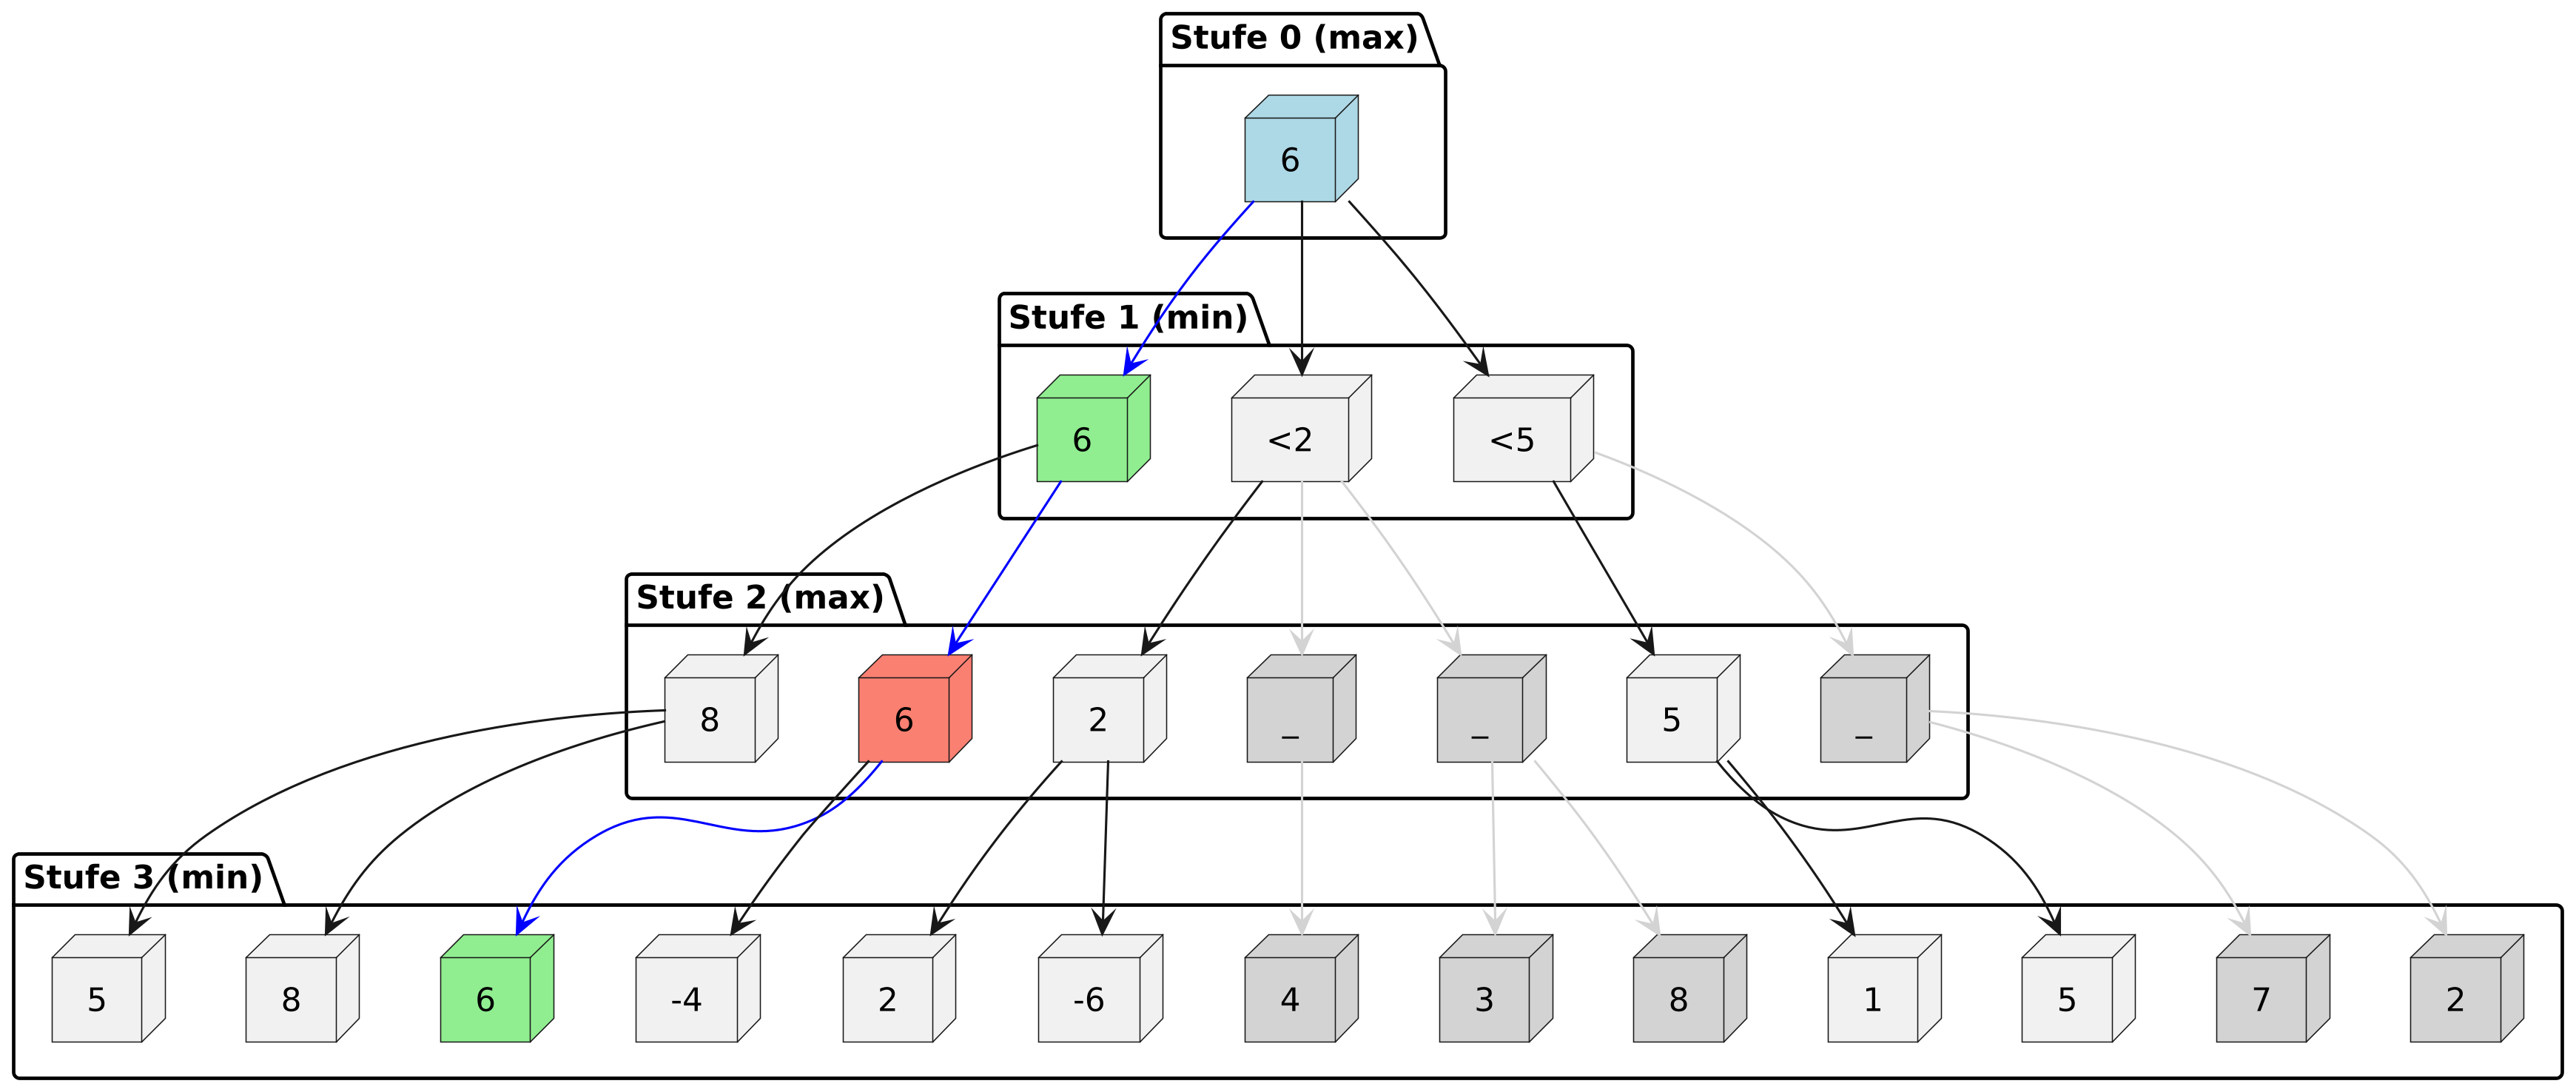
\includegraphics[width=\linewidth]{generated-diagrams/general-alpha-beta-tree-example-end}
    \caption{Minimax Alpha-Beta Beispielbaum - Zusammengefasst}
    \label{fig:minimax-alpha-beta-tree-end}
\end{figure}

\section{Heuristiken}

\section{Performance Verbesserungen}